%% LyX 2.0.2 created this file.  For more info, see http://www.lyx.org/.
%% Do not edit unless you really know what you are doing.
\documentclass[english]{article}
\usepackage[T1]{fontenc}
\usepackage[latin9]{inputenc}
\usepackage{float}
\usepackage{textcomp}
\usepackage{graphicx}
\usepackage{babel}
\begin{document}

\title{Test of renormalisation group transformation for Ising model in 1D}

\maketitle
This is short theoretical explanation of the test: \textbf{IsingTestRenormGroup1D.h}.


\section{Idea of renormalisation group}

\medskip{}


When one is near a critical point it is very difficult to compute
the partition function numerically or by various expansion techniques.
This is because of the presence of many length scales in the system.
At high $T$, there is only short-range order, the spins form small
clusters. The correlation length (approximately equal to the linear
size of the largest cluster) is small. Close $T_{C}$ somewhat larger
patches in which most of the spins are lined up in the same direction
begin to develop. When the system reaches $T_{C}$ , these patches
expand to infinite size, but fluctuations of smaller scale persist.
At the critical temperature, spins form clusters at all lengthscales,
including one infinite-size cluster (which cannot be seen on a finite
system, but we know that the correlation length has to diverge at
$T_{C}$). As a result, all scales of length must be included in a
theoretical description .

In the theory of phase transitions , one is interested in the large
distance behaviour or macroscopic properties of physical observables
near the transition temperature $T=T_{C}$. At the critical temperature,
the correlation length, which defines the scale on which correlations
above $T_{C}$ decay exponentially, diverges and the correlation functions
decay only algebraically. This gives rise to non-trivial large distance
properties that are, to a large extent, independent of the short distance
structure, a property called universality. 

\textbf{Renormalisation group (RG)} is a mathematical method that
allows systematic investigation of the changes of a physical system
as viewed at different distance scales. As the scale varies, it is
as if we are changing magnifying glass we observe the system through.
The system at one scale will generally be seen to consist of self-similar
copies of itself when viewed at a smaller scale, with different parameters
describing the components of the system. The components, or fundamental
variables, may relate to atoms, elementary particles, atomic spins,
etc. The parameters of the theory typically describe the interactions
of the components. These may be variable \textquotedbl{}couplings\textquotedbl{}
which measure the strength of various forces.

The method is based on averaging the components of the system over
some blocks, e.g. in the 1D Ising model we build blocks of few neighbouring
spins and assign a spin to them (following specific rule for that
- like majority rule). That operation changes the correlation length
allowing us to look at the system from ``further away''. We might
apply the operation recursively.

Above $T_{C}$, there is no long-range order, spins form random \textquotedblright{}up\textquotedblright{}
and \textquotedblright{}down\textquotedblright{} clusters. Under each
transformation, the correlation length (expressed in units of the
new unit cell) decreases, the clusters become smaller and smaller
as if the temperature were higher, but they never disappear. Decrease
of the correlation length under successive transformations is an extremely
useful property because it makes the fluctuations uncorrelated and
we can solve the system using an approximate theory to calculate the
properties in that region and then transform back to the original
lattice.


\section{Method}

We consider 1-dimensional Ising model: chain of spins interacting
only with their nearest neighbours at some set temperature $T$. We
investigate system near the critical point, so in 1-dimensional case$T$
should be near 0 K.

Now we want to recursively average over short distance degrees of
freedom. We divide the chain into blocks of 3 spins and assign each
block a spin resulting from majority rule (block spin \textquotedblright{}up\textquotedblright{}
if the majority of the spins in the block is \textquotedblright{}up\textquotedblright{},
and vice versa).:

\[
S=sgn(\sum_{i=1}^{3}S_{i}).
\]


In this way the length scale of the lattice is changed by a factor
3 each time. This is a \textquotedblright{}real-space block-spin renormalization-group
transformation\textquotedblright{}.

Quantity which will show us the results of renormalisation group transformation
is the correlation length, which is:

\[
\langle S_{i};S_{j}\rangle=\langle S_{i}S_{j}\rangle-\langle S_{i}\rangle\langle S_{j}\rangle.
\]


It shows us how much the two spins $S_{i}$ and $S_{j}$ are correlated.
If the spins are independent then this quantity will be zero. Typically
this quantity decays exponentially as | i \textminus{} j |\textrightarrow{}\ensuremath{\infty}
for all temperatures but critical temperature:

\[
\langle S_{i};S_{j}\rangle\propto\exp(-l/\xi)
\]


where $l=|i-j|$ and $\xi$ is a correlation length. Infinite chain
limit of the correlation function exists and is given by:

\[
\langle S_{i};S_{j}\rangle=(\tanh(\beta))^{l}
\]


where $\beta=1/k_{B}T$. So the correlation length is given by:

\[
\xi=\frac{-1}{\ln(\tanh(\beta))}.
\]



\section{Tests}

In \textit{IsingTestRenormGroup1D.h }we test renormalisation group
transformation od 1D Ising chain. We apply recursively operation of
averaging on blocks of 3 spins. We calculate spin-spin correlations
and using formula\textbf{ $\langle S_{i};S_{j}\rangle=(\tanh(\beta'))^{l}$
}we get new interaction constants $\beta'$ for shorter chains and
out temperature $T'=1/\beta'$. We plot dependence of calculated $T$'
on length of chain (Fig. 1). We can see $T$' increase with decrease
of chain length. That means that with each renormalisation step we
wander off further from the critical point which is at 0 K. The initial
temperature of the simulation was 1 K.

\begin{center}
\begin{figure}[H]
\begin{centering}
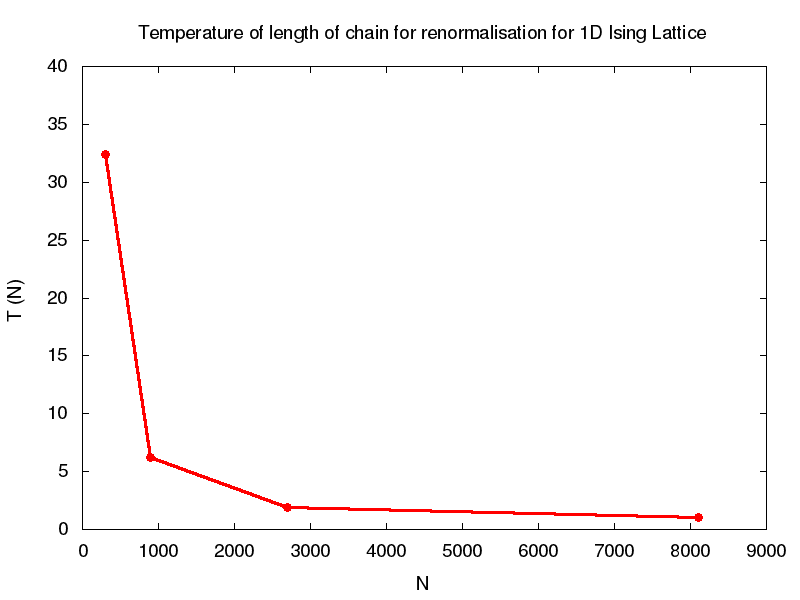
\includegraphics[scale=0.3]{IsingTestRenormGroup1D}
\par\end{centering}

\caption{Temperature in function of chain length.}
\end{figure}

\par\end{center}

Additionally we plot (Fig.2) interaction constant $\beta'=1/T'$ after
one step of renormalisation in function of initial $\beta=1/T$ (for
change of chain length $900\rightarrow300$). For comparison we add
$\beta'=\beta$ line. We can see $\beta'$ after renormalisation is
always smaller than $\beta$ and it is getting nearer $\beta'=\beta$
line for higher temperatures. This result is consistent with similar
results appearing in the literature.

\begin{figure}[H]
\begin{centering}
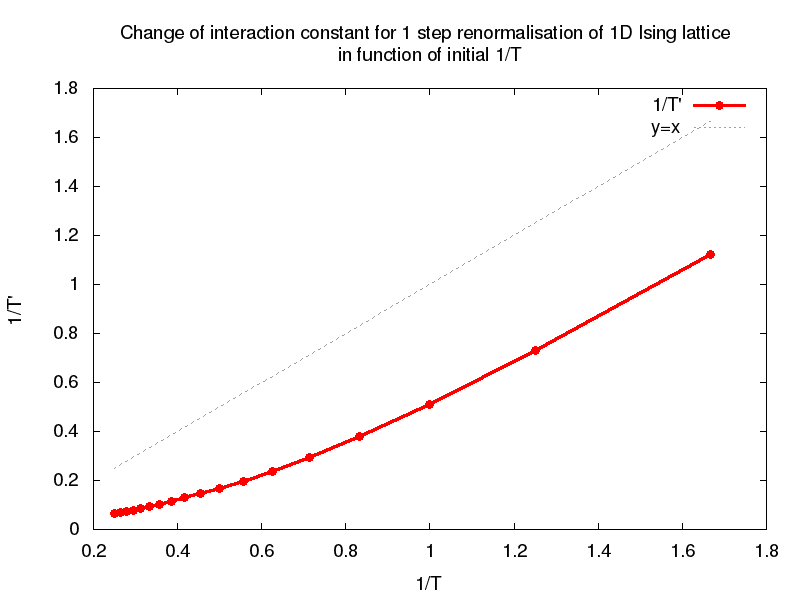
\includegraphics[scale=0.3]{IsingTestRenormGroup1D_b}
\par\end{centering}

\caption{Change of interaction constant $\beta'=1/T'$ after 1 step of renormalisation
in function of initial $1/T$.}


\end{figure}



\section{Comment on 2D model}

We do not test renormalisation group transformation on 2-dimensional
Ising model, however the procedure in that case would be similar.
We might divide 2D lattice into blocks 3x3 and apply majority rule
again. Our expectation would not be entirely the same as in 1-dimensional
case. We know that further from critical point correlations between
more distant spins become less important. As in 2D we have critical
behaviour at some non-zero temperature $T_{c}$, the temperature calculated
from spin correlation function will wander off $T_{c}$:
\begin{itemize}
\item in direction of $\infty$ if we start from $T>T_{c}$,
\item in direction of $0$ if we start from $T<T_{c}$.\end{itemize}

\end{document}
